\chapter{On Formal Feature Attribution and Its Approximation}\label{chap:ffa}


This chapter is based on:
\begin{itemize}
	\item Jinqiang Yu, Alexey Ignatiev, and Peter J. Stuckey. On Formal Feature Attribution and Its
Approximation. \emph{arXiv preprint arXiv:2307.03380,} 2023.
\end{itemize}

Serving as the alternative of model-agnostic XAI methods, 
formal XAI~(FXAI) approaches suffer from their own drawbacks,
such as scalability issues and the need to construct a logical representation
of ML models.
%
Also, formal explanations are often larger compared to their model-agnostic counterparts
as they do not take into account the reasoning about~(unknown) data distributions.
%
Lastly, and notably, FXAI approaches have not been applied to address feature attribution problems.
%
Motivated by the aforementioned limitations, this chapter introduces a 
novel formal method to generate feature attribution, 
leveraging the achievements of established FXAI techniques~\cite{msi-aaai22}.
%
Through exhaustive enumeration of all AXp's, we can define formal feature attribution~(FFA) as
the proportion of occurrences of a given feature within these AXp's.
%
Arguably, computing formal feature attribution is hard for the second level of the polynomial hierarchy.
%
While computing \emph{exact} FFA can be challening,
this chapter demonstrates that existing anytime formal explanation enumeration techniques can be
effectively used to approximate FFA.
%
Empirical results conduced on publicly accessible tabular and image datasets
show the practical effectiveness of the proposed method and its advantage
over SHAP and LIME, as well as in a real-world application of XAI in the field of 
software engineering~\cite{mcintosh2017fix,pornprasit2021pyexplainer}.


%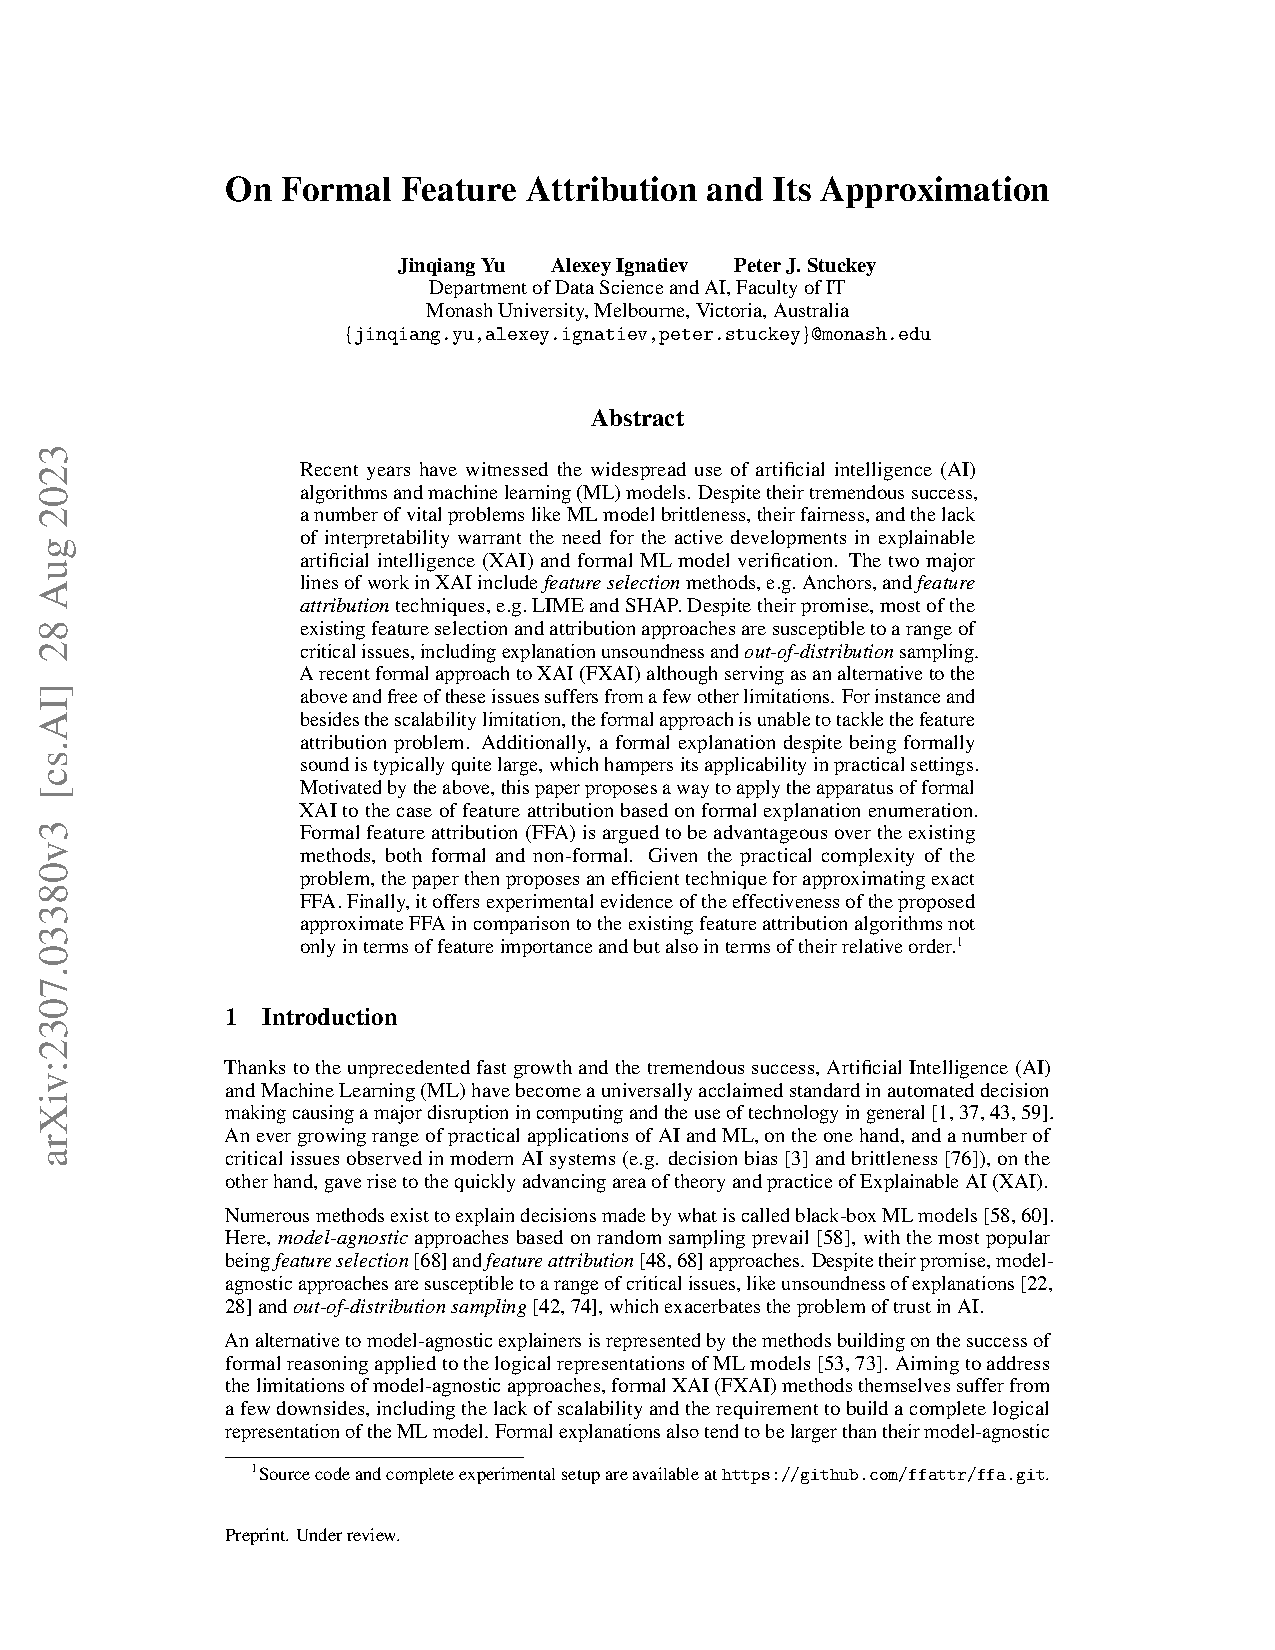
\includepdf[pages=-, offset=75 -75]{papers/ffa.pdf}
